\documentclass[10pt,aspectratio=169]{beamer}
\usetheme[progressbar=none,numbering=none]{metropolis}
\usepackage[T1]{fontenc}
\usepackage{amsmath,amssymb,booktabs}
\usepackage{graphicx}
\usepackage{tikz}
\usetikzlibrary{positioning}
\usepackage{pgfplots}
\usepackage{array}
\pgfplotsset{compat=1.18}
\definecolor{NavyBlue}{HTML}{002145}
\definecolor{AccentBlue}{HTML}{0055B7}
\definecolor{LightBlue}{HTML}{EDF3FB}
\definecolor{GraphGray}{HTML}{667685}
\definecolor{UpOrange}{HTML}{D97727}
\definecolor{Teal}{HTML}{13929A}
\definecolor{BadRed}{HTML}{B6464B}
\setbeamercolor{normal text}{fg=NavyBlue,bg=white}
\setbeamercolor{frametitle}{fg=white,bg=NavyBlue}
\setbeamercolor{title}{fg=NavyBlue}
\setbeamercolor{alerted text}{fg=AccentBlue}
\setbeamertemplate{navigation symbols}{}
\setbeamertemplate{footline}{}
\setbeamersize{text margin left=8mm,text margin right=8mm}
\newcommand{\eyebrow}[1]{{\footnotesize\color{GraphGray}#1}\par\vspace{0.07cm}}
\newcommand{\bigpoint}[1]{{\large\bfseries #1}\par}
\newcommand{\softbox}[1]{\colorbox{LightBlue}{\parbox{0.93\linewidth}{\vspace{0.10cm}#1\vspace{0.10cm}}}}
\newcommand{\citenote}[1]{{\par\noindent\parbox{\linewidth}{\tiny\color{GraphGray}#1}\par}}
% Auto-generated by scripts/build_presentation.py -- DO NOT EDIT.
% Generated 2026-10-30 from the backtest engine
%   (capital 10,000, target DTE 30, r 1.0%, q 1.3%).
% Referenced by presentation/slides.tex via % Auto-generated by scripts/build_presentation.py -- DO NOT EDIT.
% Generated 2026-10-30 from the backtest engine
%   (capital 10,000, target DTE 30, r 1.0%, q 1.3%).
% Referenced by presentation/slides.tex via % Auto-generated by scripts/build_presentation.py -- DO NOT EDIT.
% Generated 2026-10-30 from the backtest engine
%   (capital 10,000, target DTE 30, r 1.0%, q 1.3%).
% Referenced by presentation/slides.tex via \input{generated/results}.
\newcommand{\TotalReturn}{-96.0\%}
\newcommand{\MaxDrawdown}{-96.1\%}
\newcommand{\WinRate}{25\%}
\newcommand{\TradeCount}{12}
\newcommand{\FinalValue}{\$402.01}
\newcommand{\NetPnlSum}{-\$9{,}597.98}
\newcommand{\WinCount}{3}
\newcommand{\LossCount}{9}
.
\newcommand{\TotalReturn}{-96.0\%}
\newcommand{\MaxDrawdown}{-96.1\%}
\newcommand{\WinRate}{25\%}
\newcommand{\TradeCount}{12}
\newcommand{\FinalValue}{\$402.01}
\newcommand{\NetPnlSum}{-\$9{,}597.98}
\newcommand{\WinCount}{3}
\newcommand{\LossCount}{9}
.
\newcommand{\TotalReturn}{-96.0\%}
\newcommand{\MaxDrawdown}{-96.1\%}
\newcommand{\WinRate}{25\%}
\newcommand{\TradeCount}{12}
\newcommand{\FinalValue}{\$402.01}
\newcommand{\NetPnlSum}{-\$9{,}597.98}
\newcommand{\WinCount}{3}
\newcommand{\LossCount}{9}

\begin{document}

\begin{frame}[plain]
\vspace{1.06cm}
{\fontsize{29}{33}\selectfont\bfseries\color{NavyBlue}SPY Long Straddle Backtest}\par
\vspace{0.28cm}
{\color{AccentBlue}\rule{2.15cm}{1.5pt}}\par
\vspace{0.44cm}
{\large\bfseries Pavel Buklemishev}\par
\vspace{0.09cm}

\vfill
{\normalsize\bfseries Prepared for Z1 Tech}\par
\vspace{0.16cm}
{\small\href{https://github.com/radvect/spy-long-straddle-backtest}{\color{AccentBlue}\underline{github.com/radvect/spy-long-straddle-backtest}}}\par
\vspace{0.34cm}
\end{frame}

\begin{frame}{AI Assistance \& Scope}
\vspace{0.30cm}
{\large\bfseries AI Assistance}\par
\vspace{0.20cm}
ChatGPT and Claude assisted with software development and preparation of this presentation.\par

\vspace{0.95cm}
{\large\bfseries Scope of This Work}\par
\vspace{0.20cm}
This project focuses on the formulation, implementation, and computational validation of a model-based options backtest.\par
\vspace{0.34cm}
Some financial details are simplified so that I can explain the project in mathematical terms.\par
\vfill
{\bfseries All results depend on the assumptions of the model.}\par
\vspace{0.18cm}
\end{frame}


\begin{frame}{Long Straddle: From Contracts to a Payoff}
\vspace{-0.06cm}
\begin{columns}[T,onlytextwidth]
\begin{column}{0.51\textwidth}
\eyebrow{CALL + PUT, ONE STRIKE $K$, ONE EXPIRY $T$}
{\small SPY tracks the S\&P 500. The \textbf{strike} $K$ is the fixed price in the contract. A \textbf{call} allows buying SPY at $K$; a \textbf{put} allows selling at $K$. Both expire at $T$, when SPY has price $S_T$.}\par
\vspace{0.02cm}
{\small\bfseries Call and put values at expiration (per share)}
\vspace{-0.10cm}
\[
\begin{aligned}
C_T &= \max(S_T-K,0),\\[-1mm]
P_T &= \max(K-S_T,0).
\end{aligned}
\]
\vspace{-0.12cm}
\[
\boxed{C_T+P_T=|S_T-K|}
\]
\vspace{0.02cm}
{\small\bfseries Net profit or loss for one straddle}
\vspace{-0.10cm}
\[
\boxed{\Pi_T=100(|S_T-K|-C_0-P_0)-F}
\]
\vspace{-0.06cm}
{\footnotesize $C_0$ and $P_0$ are purchase prices per share; $F$ is the total trading cost. Each contract covers 100 shares.}
\end{column}
\begin{column}{0.46\textwidth}
\eyebrow{ILLUSTRATIVE PAYOFF}
{\small\bfseries Example: $K=\$500$; purchase price plus fees $=\$12$ per share}\par
\vspace{0.06cm}
\begin{tikzpicture}
\begin{axis}[
 width=\linewidth,height=4.8cm,
 axis lines=left,axis line style={GraphGray,thin},
 xmin=468,xmax=532,ymin=-16,ymax=23,
 xlabel={SPY price at expiry (\$)},ylabel={Profit/share (\$)},
 label style={font=\scriptsize},tick label style={font=\scriptsize},
 xtick={470,488,500,512,530},ytick={-12,0,20},
 grid=major,grid style={GraphGray!12},
 clip=false]
 \addplot[GraphGray!70,thin,domain=470:530]{0};
 \addplot[AccentBlue,very thick,domain=470:500]{500-x-12};
 \addplot[AccentBlue,very thick,domain=500:530]{x-500-12};
 \addplot[only marks,mark=*,mark size=1.7pt,AccentBlue] coordinates {(488,0)(500,-12)(512,0)};
 \node[font=\scriptsize,anchor=south west,fill=white,inner sep=1pt] at (axis cs:471,3){\$488};
 \node[font=\scriptsize,anchor=south east,fill=white,inner sep=1pt] at (axis cs:528,3){\$512};
\end{axis}
\end{tikzpicture}
\vspace{-0.15cm}
{\scriptsize\color{GraphGray}Break-even prices: $K\pm\$12$. Maximum loss: $\$12$ per share.}
\end{column}
\end{columns}
\end{frame}






\begin{frame}{Strategy: Four Rules}
\vspace{0.20cm}
{\large\bfseries Repeat the same trade every month.}\par
\vspace{0.32cm}
\begin{enumerate}\setlength{\itemsep}{0.38cm}
\item \textbf{Buy:} one call and one put with the same strike, closest to the current SPY price.
\item \textbf{When:} select an entry date about 30 days before a monthly expiration (allowed DTE: 21--45 days); adjust for market holidays.
\item \textbf{Exit:} hold the position until expiration and calculate its payoff.
\item \textbf{Constraint:} one straddle at a time. Skip a trade if it cannot be purchased with available cash.
\end{enumerate}
\end{frame}

\begin{frame}{Pricing and Data}
\vspace{0.19cm}
{\large\bfseries The payoff is known at expiration. We must estimate the purchase price.}\par
\vspace{0.34cm}
\begin{enumerate}\setlength{\itemsep}{0.37cm}
\item \textbf{Pricing model.} Black--Scholes estimates the call and put purchase prices from the SPY price, strike, time remaining and a volatility input. Full equations are in Appendix A.
\item \textbf{Historical prices.} We use daily SPY prices from 2020--2025 to simulate how the strategy would behave.
\item \textbf{Volatility estimate.} VIX (Cboe Volatility Index) summarizes the market's expectation of S\&P 500 price fluctuations over approximately 30 days. We use VIX/100 as an approximate annual volatility input.
\end{enumerate}
\vspace{0.16cm}
\softbox{\small Prices of SPY and VIX are observed; prices of the options are calculated. The default annual risk-free rate is 1.0\% and dividend yield is 1.3\%.}
\vspace{0.14cm}
{\small Model reference: \href{https://doi.org/10.1086/260062}{\textcolor{AccentBlue}{Black \& Scholes (1973), \emph{Journal of Political Economy}}}.}
\end{frame}



\begin{frame}{Backtest Algorithm}
\vspace{0.16cm}
{\large\bfseries Follow the data in chronological order.}\par
\vspace{0.30cm}
\begin{center}
\begin{tikzpicture}[node distance=0.18cm,every node/.style={font=\small},>=stealth]
\tikzstyle{pnode}=[draw=AccentBlue,very thick,rounded corners=2pt,minimum height=0.80cm,minimum width=2.65cm,align=center,fill=LightBlue]
\node[pnode](a){SPY and VIX\\data};
\node[pnode,right=of a](b){Estimate\\option prices};
\node[pnode,right=of b](c){Apply rule\\update cash};
\node[pnode,right=of c](d){Record\\portfolio value};
\draw[->,thick,AccentBlue](a)--(b);\draw[->,thick,AccentBlue](b)--(c);\draw[->,thick,AccentBlue](c)--(d);
\end{tikzpicture}
\end{center}
\vspace{0.45cm}
\[
\boxed{\text{Portfolio value}=\text{Cash}+\text{Value of any open position}}
\]
\vspace{0.21cm}
\begin{itemize}\setlength{\itemsep}{0.18cm}
\item At entry, record the chosen strike, expiration, purchase price and trading costs.
\item At expiration, settle the position using the payoff formula from the mathematical slide.
\item Record portfolio value and drawdown on every date.
\end{itemize}
\end{frame}


\begin{frame}{Dashboard: Controls and Summary}
\vspace{-0.05cm}
\begin{center}
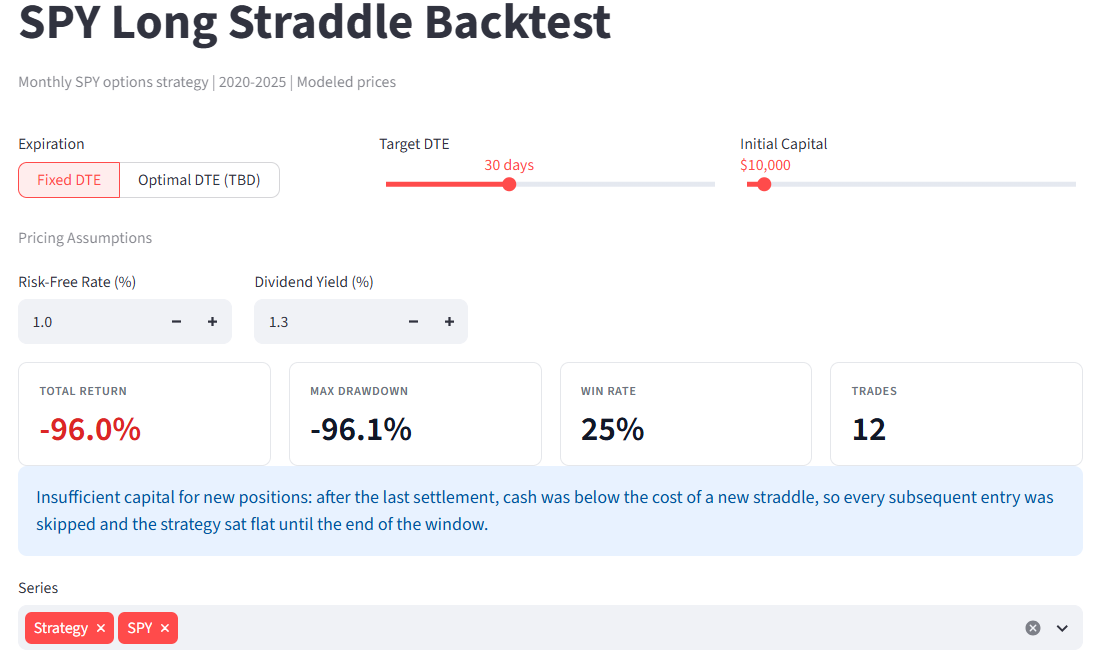
\includegraphics[width=0.96\linewidth,height=6.65cm,keepaspectratio]{figures/top_dashboard_complete.png}
\end{center}
\end{frame}

\begin{frame}{Dashboard: Trade History}
\vspace{-0.04cm}
\begin{center}
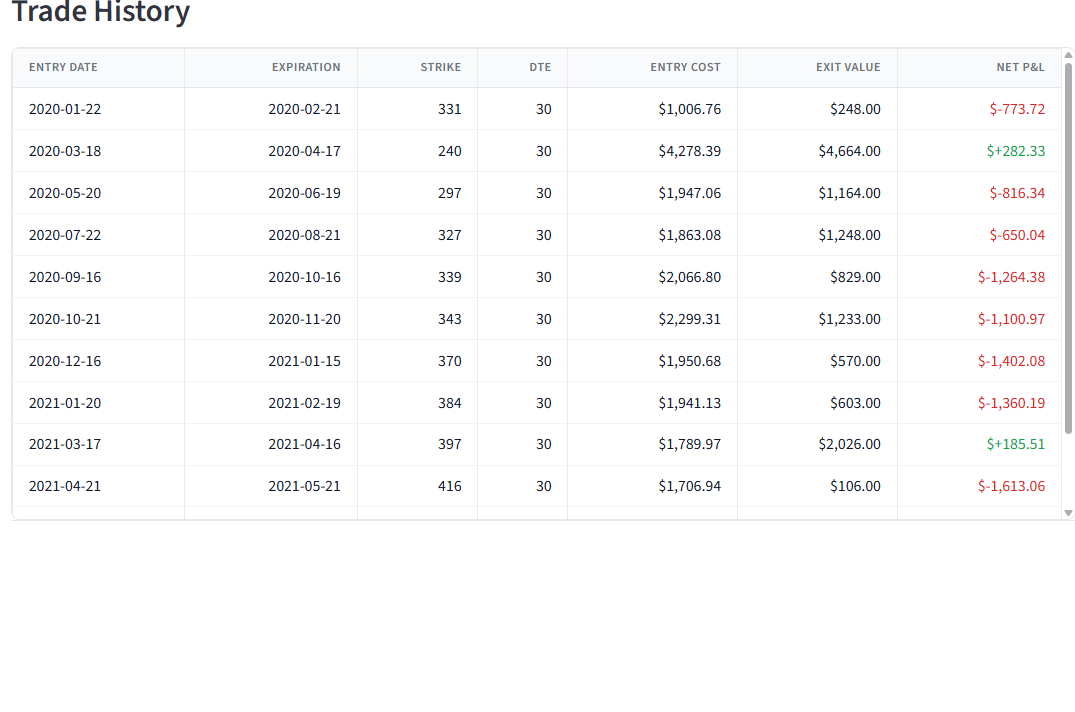
\includegraphics[width=0.96\linewidth,height=6.60cm,keepaspectratio]{figures/trade_history_cropped.png}
\end{center}
\end{frame}

\begin{frame}{Backtest Results}
\vspace{-0.06cm}
\eyebrow{JAN 2020--DEC 2025 \quad | \quad INITIAL CAPITAL \$10,000 \quad | \quad TARGET 30 DTE}
\begin{columns}[T,onlytextwidth]
\begin{column}{0.72\textwidth}
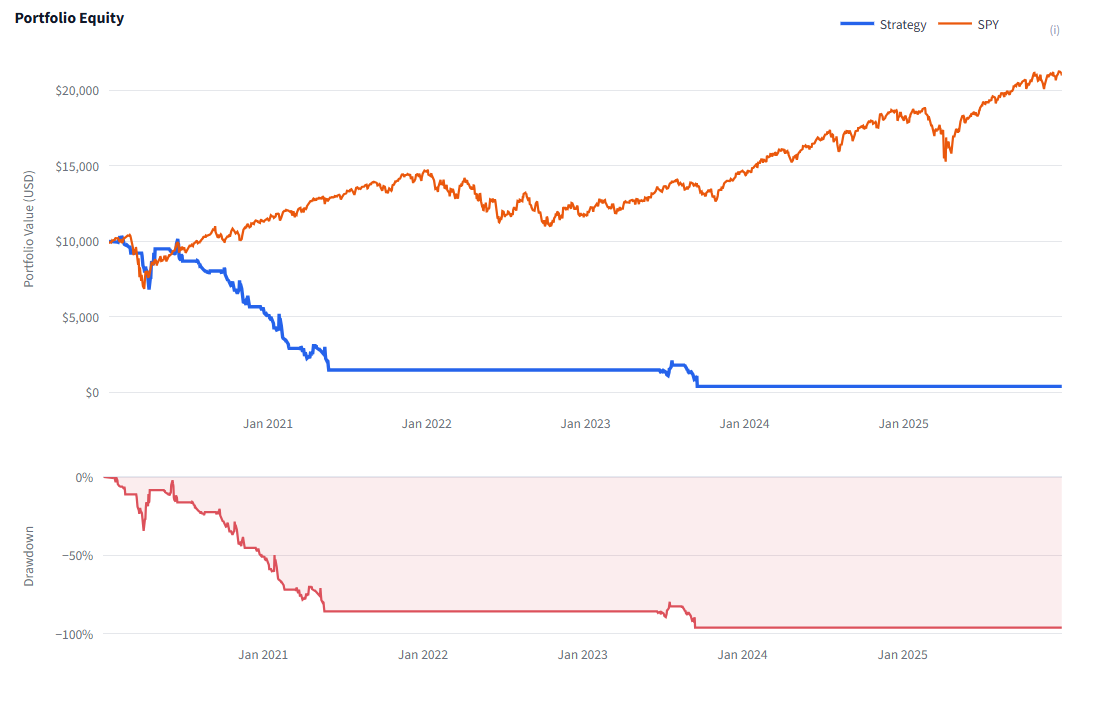
\includegraphics[width=\linewidth,height=5.56cm,keepaspectratio]{figures/equity_drawdown_cropped.png}
\end{column}
\begin{column}{0.26\textwidth}
\vspace{0.10cm}
\eyebrow{TOTAL RETURN}
{\fontsize{23}{25}\selectfont\bfseries\color{BadRed}\TotalReturn}\par
\vspace{0.20cm}
\eyebrow{MAXIMUM DRAWDOWN}
{\fontsize{23}{25}\selectfont\bfseries\color{BadRed}\MaxDrawdown}\par
\vspace{0.20cm}
\eyebrow{WIN RATE}
{\fontsize{23}{25}\selectfont\bfseries\WinRate}\par
\vspace{0.20cm}
\eyebrow{TRADES}
{\fontsize{23}{25}\selectfont\bfseries\TradeCount}\par
\end{column}
\end{columns}
\end{frame}

\begin{frame}{What Do These Results Tell Us?}
\vspace{0.10cm}
{\large\bfseries Most of the completed straddles did not recover their purchase cost.}\par
\vspace{0.42cm}
\begin{columns}[T,onlytextwidth]
\begin{column}{0.49\textwidth}
\eyebrow{RESULT OF 12 TRADES}
\begin{tikzpicture}[x=1cm,y=1cm]
\node[anchor=west,font=\small] at (0,2.65) {Unprofitable: \LossCount};
\fill[BadRed] (0,1.95) rectangle (5.3,2.41);
\node[anchor=west,font=\small] at (0,1.35) {Profitable: \WinCount};
\fill[Teal] (0,0.66) rectangle (1.77,1.12);
\end{tikzpicture}
\end{column}
\begin{column}{0.46\textwidth}
\eyebrow{FINAL PORTFOLIO VALUE}
{\fontsize{25}{27}\selectfont\bfseries \FinalValue}\par
\vspace{0.16cm}
{\small The \TradeCount recorded trade profits and losses sum to $\NetPnlSum$ from an initial \$10,000.}\par
\vspace{0.34cm}
\eyebrow{WHY DOES THE EQUITY CURVE FLATTEN?}
{\small Once available funds became too small for another straddle, new entries were skipped.}\par
\end{column}
\end{columns}
\end{frame}

\begin{frame}{Validation \& Testing}
\vspace{0.10cm}
{\large\bfseries Check formulas first, then the complete backtest.}\par
\vspace{0.30cm}
\begin{enumerate}\setlength{\itemsep}{0.28cm}
\item \textbf{Unit tests: mathematical functions.} Black--Scholes put--call parity and price bounds; ATM strike selection; expiration and DTE rules.
\item \textbf{Integration tests: full trade.} Entry, cost deduction, the 100-share multiplier, expiration payoff, and portfolio accounting.
\item \textbf{Scenario tests: known market paths.} Constant prices, large moves, market holidays, and insufficient funds.
\item \textbf{Regression tests: repeatable calculations.} Fixed synthetic input data, portfolio-value reconciliation, and performance statistics.
\end{enumerate}
\vfill
\softbox{\small \textbf{Timing check:} verify that a trade never uses data that would become available only after execution.}
\end{frame}

\begin{frame}{Conclusion, Limitations and Next Steps}
\vspace{0.15cm}
\begin{columns}[T,onlytextwidth]
\begin{column}{0.47\textwidth}
\eyebrow{OBSERVED RESULT}
\bigpoint{This fixed strategy lost money}
\vspace{0.17cm}
{\small Over the recorded period, the straddle strategy performed worse than buying and holding SPY.}\par
\vspace{0.34cm}
\eyebrow{MODEL LIMITATIONS}
\begin{itemize}\setlength{\itemsep}{0.16cm}
\item Option prices are estimated rather than observed.
\item VIX is only an approximation for the volatility of each option.
\item Black--Scholes omits early exercise and sudden price jumps.
\end{itemize}
\end{column}
\begin{column}{0.47\textwidth}
\eyebrow{FUTURE WORK}
\bigpoint{Improve the model and the experiment}
\vspace{0.20cm}
\begin{itemize}\setlength{\itemsep}{0.28cm}
\item Compare modeled option prices with historical option quotes.
\item Compare volatility models and test assumptions about trading costs.
\item Add parameter-sensitivity plots and alternative exit rules to the dashboard.
\end{itemize}
\end{column}
\end{columns}
\vfill
{\large\bfseries\color{AccentBlue}Live dashboard demonstration.}\par
\end{frame}

\appendix

\begin{frame}{Appendix A: Black--Scholes With Dividend Yield}
\vspace{0.08cm}
\[
\begin{aligned}
C_t &= S_t e^{-q\tau}\Phi(d_1)-K e^{-r\tau}\Phi(d_2),\\[0.12cm]
P_t &= K e^{-r\tau}\Phi(-d_2)-S_t e^{-q\tau}\Phi(-d_1),
\end{aligned}
\]
\[
d_1=\frac{\ln(S_t/K)+(r-q+\sigma^2/2)\tau}{\sigma\sqrt{\tau}},
\qquad d_2=d_1-\sigma\sqrt{\tau}.
\]
\vspace{0.06cm}
\softbox{\small\bfseries Consistency identity: \quad $C_t-P_t=S_t e^{-q\tau}-Ke^{-r\tau}$ \quad (put--call parity).}\par
\vspace{0.26cm}
{\small $C_t,P_t$: call and put prices at time $t$; $S_t$: SPY price; $K$: strike; $\tau$: years to expiration; $\sigma$: annual volatility; $r$: interest rate; $q$: dividend yield; $\Phi$: cumulative distribution function of the standard normal distribution.}
\vfill
{\small\color{GraphGray}This model prices European-style options. SPY options allow early exercise.}\par
\vspace{0.12cm}
{\footnotesize References:
\href{https://doi.org/10.1086/260062}{\textcolor{AccentBlue}{Black \& Scholes (1973)}};
\href{https://doi.org/10.2307/3003143}{\textcolor{AccentBlue}{Merton (1973), dividend extension}}.}
\end{frame}

\begin{frame}{Appendix B: Implementation Details}
\vspace{0.07cm}
\begin{columns}[T,onlytextwidth]
\begin{column}{0.48\textwidth}
\eyebrow{PORTFOLIO ACCOUNTING}
\begin{itemize}\setlength{\itemsep}{0.12cm}
\item At purchase, subtract $100(C_0+P_0)$ and entry costs from cash ($C_0,P_0$: purchase prices per share).
\item While holding, the position value is $100(C_t+P_t)$, where $C_t,P_t$ are current model prices per share.
\item At expiration, add $100|S_T-K|$ (minus applicable exit costs) to cash.
\item With no position, equity equals cash.
\end{itemize}
\end{column}
\begin{column}{0.48\textwidth}
\eyebrow{ASSUMPTIONS}
\begin{itemize}\setlength{\itemsep}{0.12cm}
\item VIX estimates 30-day S\&P 500 volatility. We approximate annual volatility by $\sigma_t=\mathrm{VIX}_t/100$.
\item Black--Scholes computes European-option prices. SPY options permit earlier exercise.
\item Commissions and assumed buying/selling spreads are included in trade costs.
\item Daily closing prices do not by themselves define executable trade times; timing is an important backtest limitation.
\end{itemize}
\end{column}
\end{columns}
\vfill

\end{frame}

\begin{frame}{Appendix C: Price Sensitivity}
\vspace{-0.08cm}
\begin{columns}[T,onlytextwidth]
\begin{column}{0.62\textwidth}
\eyebrow{EXAMPLE: SAME $S=K=\$500$, DIFFERENT VOLATILITY AND TIME}
{\small\bfseries Calculated price of one call + one put}\par
\vspace{0.05cm}
\begin{tikzpicture}
\begin{axis}[
 width=\linewidth,height=4.75cm,
 xmin=10,xmax=40,ymin=6,ymax=58,
 xlabel={Assumed annual volatility $\sigma$ (\%)},
 ylabel={Estimated pair price (\$/share)},
 label style={font=\scriptsize},tick label style={font=\scriptsize},
 xtick={10,15,20,25,30,35,40},ytick={10,20,30,40,50},
 grid=major,grid style={GraphGray!12},
 legend style={draw=none,fill=none,font=\scriptsize,at={(0.03,0.97)},anchor=north west},]
\addplot[Teal,thick,mark=none] coordinates {(10,9.5628) (15,14.3436) (20,19.1239) (25,23.9036) (30,28.6824) (35,33.4601) (40,38.2367)};\addlegendentry{21 days}
\addplot[AccentBlue,very thick,mark=none] coordinates {(10,11.4265) (15,17.1387) (20,22.8501) (25,28.5603) (30,34.2691) (35,39.9761) (40,45.6811)};\addlegendentry{30 days}
\addplot[UpOrange,thick,mark=none] coordinates {(10,13.9880) (15,20.9800) (20,27.9705) (25,34.9590) (30,41.9447) (35,48.9273) (40,55.9061)};\addlegendentry{45 days}
\end{axis}
\end{tikzpicture}
\end{column}
\begin{column}{0.35\textwidth}
\vspace{0.56cm}
\bigpoint{Two simple observations}
\vspace{0.25cm}
\begin{enumerate}\setlength{\itemsep}{0.33cm}
\item Greater expected price variation makes the option pair more expensive.
\item More time until expiration also increases its price in this example.
\end{enumerate}
\end{column}
\end{columns}
\vfill
{\small\color{GraphGray}Calculated model prices (not backtest returns); $r=1\%$, $q=1.3\%$.}
\end{frame}

\end{document}